

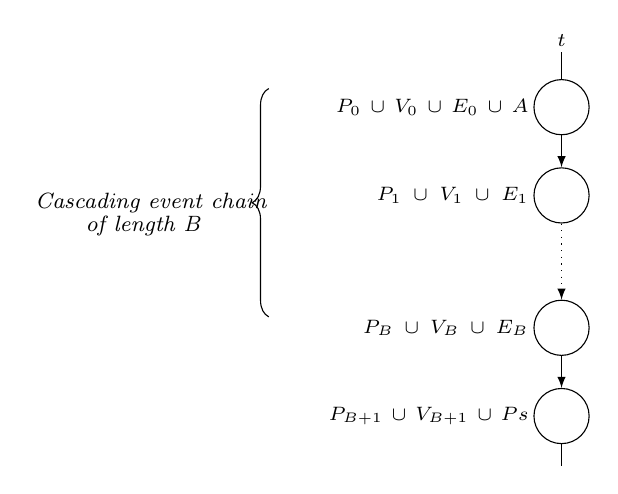
\begin{tikzpicture}[>=latex]
  \begin{scriptsize}
  \begin{scope}

  \node[align=center] (t1) at (0em,3em) {$t$};

  
  \draw (0em,2.5em) -- (0,1.25em);
 

  \node[circle, inner sep=0em, draw, minimum size=2.5em] (b0) at (0em,0) {};
  \node[align=right, text width=12em] (b0e) at (-7.5em,0) {$P_{0}\cup V_{0}\cup E_{0}\cup A$};

  \node[circle, inner sep=0em, draw, minimum size=2.5em] (b1) at (0em,-4em) {};
  \node[align=right, text width=12em] (b1e) at (-7.5em,-4em) {$P_{1}\cup V_{1}\cup E_{1}$};

  \node[circle, inner sep=0em, draw, minimum size=2.5em] (b2) at (0em,-10em) {};
  \node[align=right, text width=12em] (b2e) at (-7.5em,-10em) {$P_{B}\cup V_{B}\cup E_{B}$};
 
 \node[circle, inner sep=0em, draw, minimum size=2.5em] (bb) at (0em,-14em) {};
 
 \node[align=right, text width=12em] (bbe) at (-7.5em,-14em) {$P_{B+1}\cup V_{B+1}\cup Ps$};

  
  \draw (0em,-15.25em) -- (0,-16.25em);


  \draw[->] (b0) -- (b1);
  \draw[->, dotted] (b1) -- (b2);
  \draw[->] (b2) -- (bb);
  
  
\draw [decorate,decoration={brace,amplitude=6pt},xshift=-120pt,yshift=-90pt]
(0.5,0.5) -- (0.5,3.4) node [black,midway,xshift=-1.5cm] 
{\footnotesize $\textit{Cascading event chain}$} node [black,midway,xshift=-1.6cm, yshift=-0.3cm] 
{\footnotesize $\textit{of length B}$};

  \end{scope}
  \end{scriptsize}
\end{tikzpicture}
